\section{Atividade 4}

\subsection{Descrição do Modelo e Simulação}
Nesta atividade, analisamos um sistema de controle típico conforme descrito no diagrama de blocos abaixo. O controlador utilizado é um controlador proporcional com ganho \( K = \frac{m}{3} \). A função de transferência da planta corresponde à função de transferência da Atividade 3. O sensor é modelado por um sistema de primeira ordem com ganho \( K_s = 1 \) e constante de tempo \( T_s = \frac{m}{6} \).

\subsection{Construção do Diagrama de Blocos}
O diagrama de blocos do sistema é mostrado abaixo:
\begin{figure}[H]
    \centering
    % Inserir diagrama de blocos aqui
    % \includegraphics[width=0.7\textwidth]{path/to/diagrama_blocos.png}
    \caption{Diagrama de blocos do sistema de controle}
    \label{fig:diagrama_blocos}
\end{figure}

As funções de transferência são definidas como:
\begin{itemize}
    \item \( G_c(s) = \frac{m}{3} = \frac{10}{3} \)
    \item \( G_p(s) = \frac{1}{10 s^2 + 7 s + 5} \)
    \item \( H(s) = \frac{1}{1 + \frac{10}{6} s} = \frac{1}{1 + 1.6667 s} \)
\end{itemize}

\subsection{Função de Transferência em Malha Fechada}
A função de transferência em malha fechada \( C(s)/R(s) \) é obtida pela relação:
\[
    G_{closed}(s) = \frac{G_c(s) G_p(s)}{1 + G_c(s) G_p(s) H(s)}
\]
Substituindo as expressões das funções de transferência, temos:
\[
    G_{closed}(s) = \frac{\frac{10}{3} \cdot \frac{1}{10 s^2 + 7 s + 5}}{1 + \frac{10}{3} \cdot \frac{1}{10 s^2 + 7 s + 5} \cdot \frac{1}{1 + 1.6667 s}}
\]

Simplificando a expressão:
\[
    G_{closed}(s) = \frac{0.6 + s}{0.9 + 0.92s + 1.3s^2 + s^3}
\]

\subsection{Análise de Estabilidade pelo Critério de Routh-Hurwitz}
A análise de estabilidade é realizada utilizando o critério de Routh-Hurwitz. Os coeficientes do polinômio do denominador da função de transferência em malha fechada foram extraídos e utilizados na matriz de Routh-Hurwitz para determinar a estabilidade do sistema.

\subsubsection{Resultados da Análise de Estabilidade}
A matriz de Routh-Hurwitz calculada é:
\[
    RH\_matrix = \begin{bmatrix}
        0.9  & ... \\
        0.92 & ... \\
        1.3  & ... \\
        1    & ... \\
    \end{bmatrix}
\]

O sistema é estável, pois todos os elementos da primeira coluna da matriz de Routh-Hurwitz são positivos.

\subsection{Análise de Estabilidade para Diferentes Valores de \( K \)}
Para diferentes valores do ganho do controlador \( K \), a estabilidade do sistema foi verificada. A análise mostrou que o sistema é estável para todos os valores de \( K_p \) testados (de 1 a 10).

\subsubsection{Resultados da Resposta ao Degrau}
Abaixo, mostramos o gráfico da resposta ao degrau para diferentes valores de \( K_p \):

\begin{figure}[H]
    \centering
    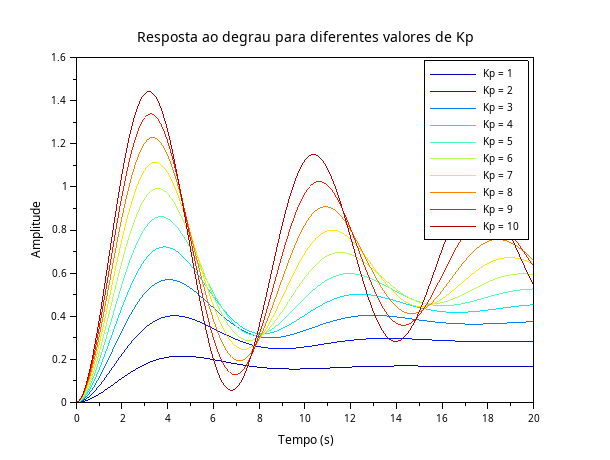
\includegraphics[width=0.7\textwidth]{4-atividade/assets/impulsos-diferentes-kp.png}
    \caption{Resposta ao degrau para diferentes valores de \( K_p \)}
    \label{fig:resposta-degrau-kp}
\end{figure}

\subsection{Conclusões}
A análise da resposta ao degrau e da estabilidade utilizando a matriz de Routh-Hurwitz mostrou que o sistema massa-mola-amortecedor controlado proporcionalmente é estável para os valores de \( K_p \) entre 1 e 10. O comportamento da resposta ao degrau varia significativamente com o ganho do controlador, como esperado, demonstrando a importância de ajustar corretamente o ganho do controlador para atingir a resposta desejada do sistema.
